\section{Визуальное представление} \label{ch3:rendering}
	Результатом вышеприведенных алгоритмов симуляции поверхности ткани является множество точек, не подходящее для визуального представления. В связи с этим возникает вопрос о том, как правильно отображать результаты работы проделанной симуляции. Назовем симуляционным мешем (simulation mesh) - множество точек, соединенных ограничениями, являющееся результатом работы симуляционного алгоритма. Мешем отрисовки (render mesh) назовем набор данных, используемых для отрисовки некоторого объекта с помощью графических систем. Меш отрисовки может быть получен одним из двух способов:
	\begin{enumerate}[1.]
		\item Взят из готовой трёхмерной модели, созданной в геометрическом редакторе. Тогда часть вершин меша отрисовки закрепляется за частицами симуляционного меша и, подобно алгоритму скелетной анимации, симуляционный меш становится \say{скелетом} для меша отрисовки. (\firef{fig:meshSkinning}).
		\item Процедурно сгенерирован на основании симуляционного меша. Тогда он может иметь более простую структуру и будет задаваться какими-либо правилами.
	\end{enumerate}
	
	\begin{figure}[ht!] 
		\center
		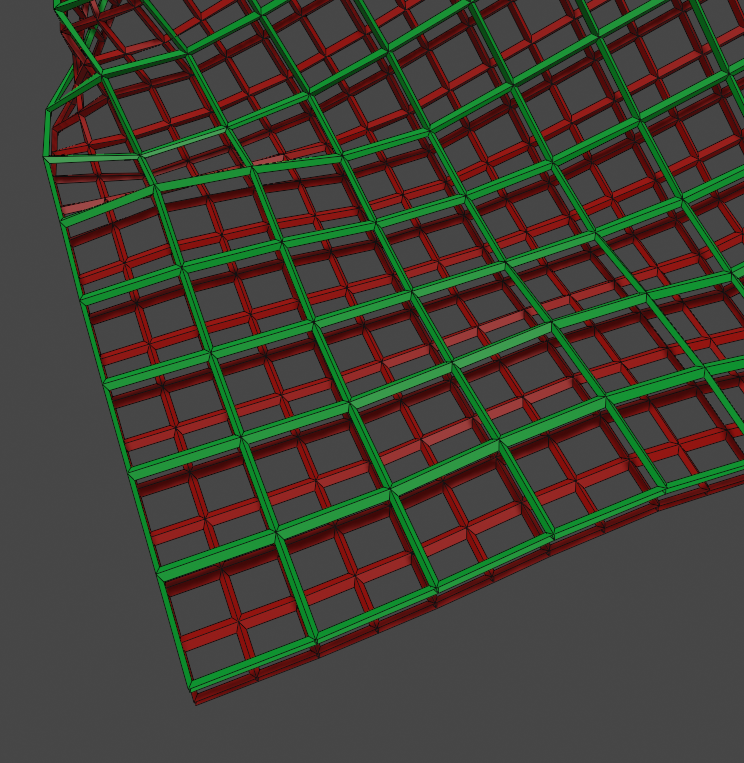
\includegraphics [scale=0.5] {my_folder/images//simrendermesh}
		\caption{Пример закрепления меша отрисовки за симуляционным мешем. Зеленым отмечен симуляционный меш, красным отмечен меш отрисовки}
		\label{fig:meshSkinning}  
	\end{figure}
	
	В рамках данной работы была разработана система процедурной генерации меша отрисовки, поддреживаемого системой визуализации "DX12Engine" \cite{me_bachelor}. Модель освещения, используемая в данной системе, относится к основанным на физической модели микрограней \cite{walter2007microfacet}, данная модель освещения также подразумевает сохраниение энергии в соответствии с \say{основным уравнением рендеринга} \cite{kajiya1986rendering}. Для этого используется двулучевая функция отражательной способности Кука-Торренса \cite{cook1982reflectance} и поправка Френеля-Шлика \cite{schlick1994inexpensive}. Для рассеянных отражений применяется модель Ламберта \cite{ikeuchi2014lambertian}, а глобальное освещение производится по методу Image-Based Lighting \cite{debevec1998rendering}.
	
	Чтобы построить меш отрисовки, который может быть отображен с использованием вышеописанной модели освещения, требуется задать следующие параметры:
	\begin{itemize}
		\item Положения вершин меша отрисовки.
		\item Индексы вершин, образуюших треугольники, для задания геометрической структуры.
		\item Вектор нормали в каждой вершине меша.
		\item Текстурные координаты в каждой вершине меша.
		\item Тангент вектор в каждой вершине меша.
		\item Карта нормалей.
		\item Коэффициент металличности.
		\item Коэффициент шероховатости.
		\item Коэффициент цвета.
	\end{itemize}
	
	Для задания положений вершин меша отрисовки используются вершины симуляционного меша. В таком случае не требуется использовать какой-либо алгоритм для задания положений вершин, не имеющих соответствия среди симуляционных вершин, так как все вершины меша отрисовки будут закрепелены за вершинами симуляционного меша.
	
	Для задания индексов вершин используется тот факт, что частицы симуляционного меша представляются в виде прямоугольной сетки (как рассказано в параграфе \ref{ch2:connect}). Таким образом, используя структурные ограничения и ограничения сдвига, можно построить два вида сетки, представленные на \firef{fig:meshConnect}.
	
	\begin{figure}[ht!] 
		\center
		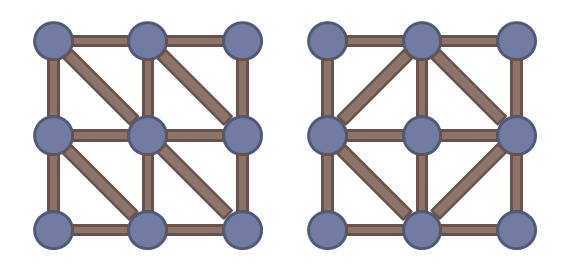
\includegraphics [scale=1] {my_folder/images//meshConnect}
		\caption{Примеры двух вариантов соединения точек меша отрисовки треугольниками.}
		\label{fig:meshConnect}  
	\end{figure}
	
	Для задания вектора нормали в вершине используется алгоритм нахождения нормали в триангулированных моделях. Согласно данному алгоритму, нормалью в вершине принято считать нормализированную сумму нормалей всех треугольников, которые задаются в том числе данной вершиной. Нетрудно заметить, что на \firef{fig:meshConnect}, левая конфигурация предполагает вычисление нормалей шести треугольников для определения нормали центральной вершины, в то время как при использовании правой конфигурации будет достаточно всего четырёх.
	
	Для задания текстурных координат можно воспользоваться тем фактом, что меш отрисовки, также как и симуляционный меш, представляет собой прямоугольную сетку. Введём систему координат вдоль этой прямоугольной сетки таким образом, чтобы крайние вершины имели координаты (0, 0), (1, 0), (0, 1), (1, 1). Для каждой вершины из оставшихся определяются текстурные координаты в соответствии с вышеупомянутой системе координат (\firef{fig:texCoord}).
	
	\begin{figure}[ht!] 
		\center
		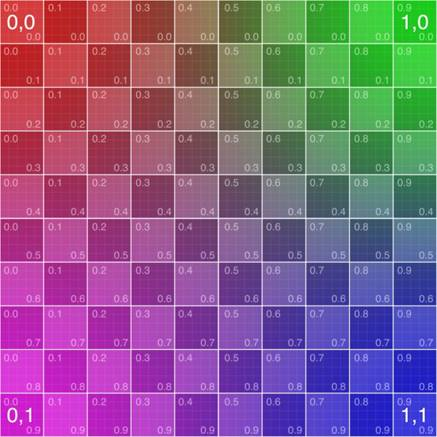
\includegraphics [scale=0.9] {my_folder/images//texCoord}
		\caption{Текстурные координаты для поверхности, заданной прямоугольной сеткой}
		\label{fig:texCoord}  
	\end{figure}
	
	Для задания тангент вектора используются сгенерированные текстурные координаты и векторы нормали в вершинах. Чтобы определить тангент вектор, для каждой вершины меша отрисовки производятся следующие операции:
	\begin{enumerate}[1.]
		\item Находится ближайшая \say{правая} вершина, исходя из представления в текстурных координатах
		\item При помощи векторного произведения между нормалью к текущей вершине и направлением на \say{правую} вершину определяется вектор бинормали
		\item Векторное произведение бинормали и нормали в результате определяет тангент вектор.
	\end{enumerate}
	
	Все остальные параметры могут быть представлены в виде текстур и найдены в сети Интернет.
	
	Построенный с помощью приведённых выше действий объект готов к использованию в системе визуализации трёхмерной компьютерной графики и может отображать результаты физической симуляции.

%% Вспомогательные команды - Additional commands
%
%\newpage % принудительное начало с новой страницы, использовать только в конце раздела
%\clearpage % осуществляется пакетом <<placeins>> в пределах секций
%\newpage\leavevmode\thispagestyle{empty}\newpage % 100 % начало новой страницы